\documentclass{article}

\usepackage[paper=a4paper,margin=0.9in]{geometry}

\usepackage{mathtools}
\usepackage{enumitem} % enumeration label options
\usepackage{amsfonts} % \mathbb
\usepackage{mathrsfs} % \mathscr
\usepackage{amsthm}
\usepackage{tikz-cd}
\usepackage{stmaryrd} % \sslash

\setlength{\parindent}{0pt}

\newtheorem*{conjecture}{Conjecture}
\newtheorem*{theorem}{Theorem}
\newtheorem*{corollary}{Corollary}
\newtheorem*{lemma}{Lemma}
\newtheorem*{proposition}{Proposition}

\theoremstyle{definition}
\newtheorem*{definition}{Definition}
\newtheorem*{example}{Example}
\newtheorem*{remark}{Remark}
\newtheorem*{exercise}{Exercise}

\DeclareMathOperator{\PGL}{PGL}
\DeclareMathOperator{\Bl}{Bl}
\DeclareMathOperator{\Spec}{Spec}
\DeclareMathOperator{\Supp}{Supp}
\DeclareMathOperator{\exc}{exc}
\DeclareMathOperator{\supp}{supp}
\DeclareMathOperator{\cosupp}{cosupp}
\DeclareMathOperator{\mld}{mld}
\DeclareMathOperator{\lct}{lct}
\DeclareMathOperator{\LCT}{LCT}
\DeclareMathOperator{\Res}{Res}
\DeclareMathOperator{\Hom}{Hom}

\newcommand{\closure}[1]{\overline{#1}}
\newcommand{\cat}[1]{\mathsf{#1}}

\newcommand{\sm}{\mathrm{sm}}
\newcommand{\Diff}{\mathrm{Diff}}

\newcommand{\U}{\mathcal{U}}
\newcommand{\M}{\mathcal{M}}
\newcommand{\I}{\mathscr{I}}
\newcommand{\J}{\mathscr{J}}
\renewcommand{\O}{\mathcal{O}}
\newcommand{\A}{\mathbb{A}}
\renewcommand{\P}{\mathbb{P}}
\newcommand{\F}{\mathbb{F}}
\newcommand{\N}{\mathbb{N}}
\newcommand{\Z}{\mathbb{Z}}
\newcommand{\Q}{\mathbb{Q}}
\newcommand{\R}{\mathbb{R}}
\newcommand{\C}{\mathbb{C}}

\title{LTCC 2023-2024: Birational Geometry}
\author{Calum Spicer}
\date{}

\begin{document}

\maketitle

\section*{Overview}

The course will assume the content of Hartshorne\footnote{With the caveat that
he doesn't remember what exactly is and isn't in Hartshorne.}. We will look at
two main topics which may initially not look hugely related to birational
geometry, but in fact encompass a lot of the important ideas.
\begin{itemize}
    \item Moduli spaces: These are schemes / algebraic spaces / stacks / e.t.c.
        associated to a collection of algebraic objects (e.g. curves, surfaces,
        sheaves, ...).

    \item Foliations: These are a clever way of decomposing a space into
        subspaces, or analogously considering fibres in a fibre space.
\end{itemize}

\section*{Singularities and adjunction}

All schemes are considered over a field $k$ of characteristic 0.

\begin{example}
    Consider $\A^2\cong\Spec k[x,y,t]/(xy-t)\xrightarrow{f}\Spec k[t]=\A^1$. For
    points $p\ne0$ in $\A^1$, the fibre $f^{-1}(p)$ is a smooth curve (a conic).
    For $p=0$ however  $f^{-1}(p)=V(xy)$ is a nodal singular curve. What does
    this say about the moduli space of curves? It says the moduli space of
    smooth curves is not proper / compact. (One might ask: why care about
    compactness for moduli spaces?)
\end{example}

\begin{exercise}
    Show that there does not exist an exact sequence
    \begin{equation*}
        0 \to \O(a) \to \Omega^1_{\P^2} \to \O(b) \to 0
    \end{equation*}
    of sheaves on $\P^2$ for any $a,b\in\Z$. As a consequence, there are no
    smooth foliations on $\P^2$.
\end{exercise}

So from looking at the simplest cases of our main topics: the moduli space of
curves, and foliations of $\P^2$, we see that singularities naturally arise.

\begin{theorem}[Hironaka]
    Let $X$ be a smooth variety over $k$ a field of characteristic 0, and let
    $\I\subseteq\O_X$ be an ideal sheaf. Then there exists a composition
    $b:X'\to X$ of blowups in smooth centres (i.e. along subvarieties which are
    smooth) contained in the singular locus of $X$, such that the cosupport of
    $b^{-1}\I=\I\cdot\O_{X'}$ is a simple normal crossings divisor.
\end{theorem}

\begin{remark}
    The cosupport of an ideal sheaf is the support of the quotient;
    $\cosupp(\J)\coloneq\supp(\O_X/\J)$.
\end{remark}

\begin{corollary}[Resolution of Singularities]
    Let $X$ be a normal variety over $k$ a field of characteristic 0. Then there
    exists a composition $b:X'\to X$ of blowups in smooth centres contained in
    the singular locus of $X$, such that $X'$ is smooth and the exceptional
    locus $\exc(b)$ is a simple normal crossings divisor. As a consequence,
    every variety is birational to a smooth variety.
\end{corollary}

\begin{proof}
    Embed $X\hookrightarrow Y$ with $Y$ smooth, which is possible because $X$ is
    a variety (Chow's lemma). Let $\pi:Y'\to Y$ be the composition of blowups
    obtained from Hironaka's lemma applied to the subvariety $X$. Then
    $\pi^{-1}(X)$ is a divisor, so at some point we must have blown up $X$.
    (Since we may assume $X$ has codimension at least 2 in $Y$.) Since we only
    blow up in smooth centres, at some point $X$ must have become smooth.
\end{proof}

The philosophy of Grothendieck is that we should study morphisms (of schemes
e.t.c.), not just the objects (schemes e.t.c.) themselves. Hironaka's theorem
tells us that we can make any morphism $X\to\Spec k$ smooth by blowing up. What
about general morphisms $f:X\to Z$?\footnote{We call a morphism smooth if it is
flat and has regular fibres.} The answer is no. Consider the example from above:
\begin{equation*}
    \A^2 \cong \Spec\frac{k[x,y,t]}{(xy-t)} \to \Spec k[t] = \A^1.
\end{equation*}
This morphism has a singularity at $(0,0)$ in $\A^2$ from the singular fibre
$V(xy)$ over $0\in\A^1$. If we blowup the origin the fibre over $0\in\A^1$
remains singular because of the exceptional divisor:
\begin{center}
    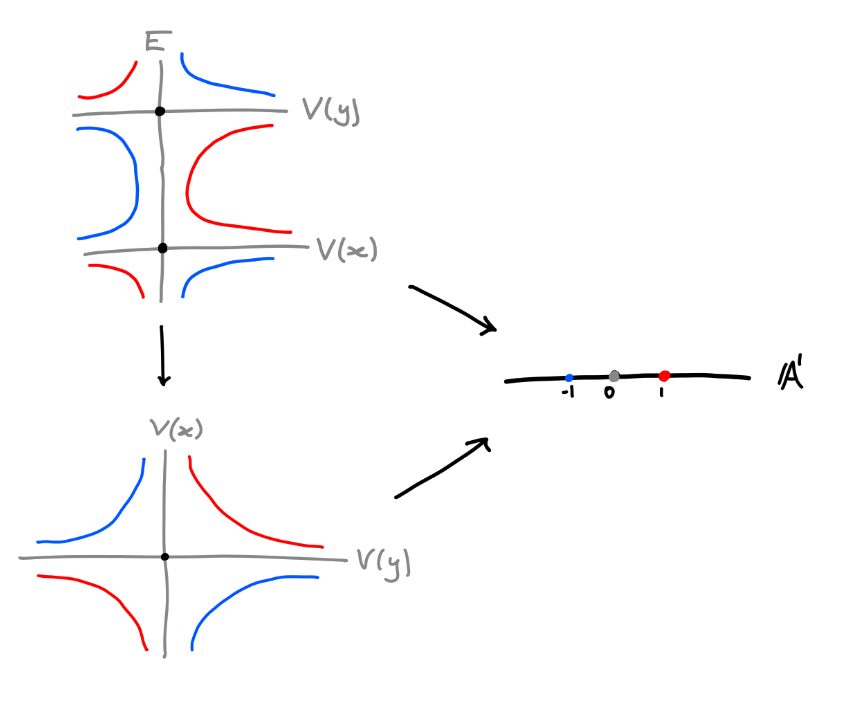
\includegraphics[scale=0.4]{hyperbola_blowup}
\end{center}
So the question becomes: what ``nice'' singularities should we allow?

\begin{definition}
    Let $f:(p,X)\to(q,Z)$ be a morphism of germs of smooth varieties. (Think of
    the germs as $\Spec\O_{X,p}$, or other possibilities.) We say $f$ is
    \emph{toroidal} if there exist \'etale / analytic / formal coordinates
    $x_1,\ldots,x_n$ and $z_1,\ldots,z_k$ such that $f$ can be written as
    \begin{equation*}
        z_{i_l} = x_1^{m_{1,i_l}}\cdots x_n^{m_{n,i_l}}
    \end{equation*}
    for some collection of indices $i_l\in\{1,\ldots,k\}$. In other words, if
    $f$ can be written as monomials. We say a morphism $f:X\to Z$ is toroidal if
    all its germs are toroidal.
\end{definition}

\begin{example}
    Smooth morphisms are toroidal, by the inverse function theorem. The map
    $\Spec k[x,y,t]/(xy-t)\to\Spec k[t]$ is toroidal, as it can be written in
    coordinates as $(u,v)\mapsto uv$.
\end{example}

\begin{remark}
    Toroidal means formally locally isomorphic to a morphism of toric varieties.
    A good short reference for toric varieties is Fulton's book ``Introduction
    to Toric Varieties''.
\end{remark}

\begin{conjecture}
    Let $f:X\to Z$ be a morphism of varieties. Then there exists a diagram
    \begin{equation*}
        \begin{tikzcd}
            &X' \ar[r,"\beta"] \ar[d,"f'"] &X \ar[d,"f"] \\
            &Z' \ar[r,"\alpha"] &Z
        \end{tikzcd}
    \end{equation*}
    such that $\alpha$ and $\beta$ are birational maps and $f'$ is toroidal.
\end{conjecture}

\begin{remark}
    We are not assuming that $f$ has connected fibres here. (Recall connected
    fibres is equivalent to $f_*\O_X=\O_Z$ by Zariski's main theorem.) This is a
    naive way of generalizing Hironaka's theorem to morphisms, taking the
    ``nice'' class of singularities to be the toroidal singularities.
\end{remark}

\begin{theorem}[Abramovich--Karu]
    The above conjecture holds if $f:X\to Z$ is projective and has connected
    fibres (i.e. $f_*\O_X=\O_Z$).
\end{theorem}

\begin{definition}
    We say $f:X\to Z$ is \emph{semi-stable} if $f$ is toroidal and the
    scheme-theoretic fibres of $f$ are reduced.
\end{definition}

\begin{example}
    We cannot always achieve semi-stability by blowups; consider again the above
    example:
    \begin{align*}
        g : \Bl_{(0,0)}\A^2 \xrightarrow{b} \A^2 &\xrightarrow{f} \A^1 \\
            (x,y) &\mapsto xy
    \end{align*}
    This is a toroidal morphism, but we have
    \begin{align*}
        g^*(0)
            &= b^*(V(xy)) \\
            &= b^*(V(x)) + b^*(V(y)) \\
            &= (b_*^{-1}(V(x))+E) + (b_*^{-1}(V(y))+E) \\
            &= b_*^{-1}(V(x)) + b_*^{-1}(V(y)) + 2E
    \end{align*}
    where $E$ is the exceptional divisor, so $g^{-1}(0)$ is not reduced (having
    multiplicity 2 along $E$).
\end{example}

\begin{remark}
    Semi-stable morphisms ``should be'' universal families over moduli spaces,
    whatever that means.
\end{remark}

\begin{conjecture}[Semi-Stable Reduction]
    Let $f:X\to Z$ be a projective morphism with connected fibres. Then there
    exists a diagram
    \begin{equation*}
        \begin{tikzcd}
            &X' \ar[r,"\beta"] \ar[dr,"f'",swap]
                &X\times_ZZ' \ar[d] \ar[r] &X \ar[d,"f"] \\
            & &Z' \ar[r,"\alpha"] &Z
        \end{tikzcd}
    \end{equation*}
    with $\alpha$ generically finite and $\beta$ birational, such that
    \begin{enumerate}[label=\arabic*)]
        \item $X'$ and $Z'$ are smooth,
        \item $f'$ is equi-dimensional, and
        \item $f'$ is semi-stable.
    \end{enumerate}
\end{conjecture}

\begin{remark}
    If we don't require $f'$ to be smooth this is ``weakly semi-stable
    reduction''.
\end{remark}

The case $\dim Z=1$ is known by work of Kempf--Kunetsu--Mumford--Saint Denis.
Weakly semi-stable reduction is known in all dimensions by Abramovich--Karu.
The case of relative dimension 1 is known by work of de Jong.

\section*{Singularities and MMP}

\begin{definition}
    Let $X$ be a smooth variety of dimension $n$. A \emph{canonical divisor}
    $K_X$ on $X$ is a Weil divisor such that
    $\O(K_X)\cong\omega_X\coloneq\Omega_X^n$, the sheaf of holomorphic
    $n$-forms. If $X$ is a normal variety, with smooth locus $X^\sm\subseteq X$
    such that $Z=X\setminus X^\sm$ has codimension at least 2 in $X$, then we
    define a canonical divisor on $X$ as the unique divisor $K_X$ such that
    $K_X|_{X^\sm}=K_{X^\sm}$.
\end{definition}

\begin{example}
    If $X$ is a smooth variety and $\theta$ is a rational $n$-form, i.e. a
    section of $\omega_X\otimes_{\O_X}K(X)$, then
    \begin{equation*}
        K_X = (\theta)_0 - (\theta)_\infty;
    \end{equation*}
    the locus of zeros minus the locus of poles gives a canonical divisor. In
    particular, for $\P^n$ we get
    \begin{equation*}
        K_{\P^n} = -(n+1)\cdot H
    \end{equation*}
    where $H$ is a hyperplane. (Take $dx_0\wedge\cdots\wedge dx_n$ on
    $\A^{n+1}$, which extends to a rational $n$-form on $\P^n$ with a pole of
    order $n+1$ along the hyperplane at infinity.)
\end{example}

\section*{Toric geometry}

\begin{definition}
    The \emph{complex torus} is $(\C^\times)^n=(\A^1\setminus\{0\})^n$. A
    \emph{toric variety} is a normal variety $X$ of dimension $n$ which contains
    the complex torus $(\C^\times)^n$ as a Zariski open subset, such that the
    action of $(\C^\times)^n$ on itself extends to an action of $(\C^\times)^n$
    on $X$.
\end{definition}

\begin{example}
    We have $\A^n\supseteq(\A^1\setminus\{0\})^n=(\C^\times)^n$. The torus
    action is given by
    $(t_1,\ldots,t_n)\cdots(x_1,\ldots,x_n)=(t_1x_1,\ldots,t_nx_n)$ which
    extends to all of $\A^n$ and even to $\P^n$. By taking products of tori and
    their actions we see that $\P^n\times\P^m$ is also toric.
\end{example}

\begin{lemma}
    Let $X$ be a toric variety. We have
    \begin{equation*}
        K_X = -\sum_{\text{$D$ torus invariant}}D,
    \end{equation*}
    where a divisor $D$ is torus invariant if for all $t\in(\C^\times)^n$ we
    have $t\cdot D=D$.
\end{lemma}

\begin{proof}
    Look at $\theta=\frac{dt_1}{t_1}\wedge\cdots\wedge\frac{dt_n}{t_n}$ on
    $(\C^\times)^n$. It has poles along the torus invariant divisors, and no
    zeros.
\end{proof}

\begin{example}
    On $\A^n$, the torus invariant divisors are the axes $\{x_i=0\}$, of which
    there are $n$. For $\P^n$ the torus invariant divisors are also the axes
    $\{x_i=0\}$, of which there are $n+1$. We again see
    \begin{equation*}
        K_{\P^n}=-\sum_{i=0}^nH=-(n+1)H.
    \end{equation*}
\end{example}

\begin{exercise}
    Which quotient singularities are toric? (Recall that a quotient singularity
    is given by $\A^n/G=\Spec k[x_1,\ldots,x_n]^G$ for $G$ a finite group.)
    % E_6,E_7,E_8 not toric, A_n toric
\end{exercise}

\section*{Canonical divisors and discrepancies}

Let $X$ be a smooth variety, and $W\subseteq X$ a smooth subvariety of
codimension $k$. Consider the blowup $b:X'\to X$ in $W$. What is the relation
between $K_X$ and $K_{X'}$? We have the exceptional divisor $E$, with
\begin{equation*}
    K_{X'} = b^*K_X + aE.
\end{equation*}

\begin{proposition}
    In the above setup, we have $a=k-1$.
\end{proposition}

\begin{proof}
    This is a local question, and everything is toroidal, and hence the setup is
    locally isomorphic to the blowup of a toric variety in a torus invariant
    centre. (Using Artin approximation.) So we are reduced to the case
    $X'\to\A^n$, where $K_{\A^n}=-\sum\{x_i=0\}$. Then
    \begin{equation*}
        -K_{X'} = \sum\{x_i=0\}' + E,
    \end{equation*}
    where $(\cdot)'$ denotes the strict transform, and
    \begin{equation*}
        -b^*\sum\{x_i=0\} = \sum\{x_i=0\}' + kE
    \end{equation*}
    since $W$ is given by $\{x_1=\cdots=x_k=0\}$.
\end{proof}

\begin{exercise}
    If $b$ is a weighted blowup, what happens to $a$?
\end{exercise}

More generally, if $b:X'\to X$ is birational we have
\begin{equation*}
    K_{X'} = b^*K_X + \sum_{\text{$E_i$ exceptional}}a(E_i,X)E_i,
\end{equation*}
where $a(E_i,X)$ are called the \emph{discrepancies}. Intuitively, smaller
discrepancies mean worse singularities.

\begin{remark}
    For a general birational morphism, we define the exceptional divisors as the
    components of the complement of the maximal domain of definition.
    Equivalently, these are the divisors $E$ in $X'$ such that $b(E)$ is not a
    divisor in $X$. The non-existence of exceptional divisors does not imply
    that the map is an isomorphism; there exist birational morphisms $X'\to X$
    with $\dim X=\dim X'=3$ contracting curves to points.
\end{remark}

\begin{example}
    Consider $C\subseteq\P^2$ a smooth curve of degree $d$, and $X\subseteq\A^3$
    the cone over $C$. (So $X=\Spec\oplus_{n=0}^\infty H^0(C,\O(n)|_C)$, or
    equivalently $X=\overline{q^{-1}(C)}$ for $q:\A^3\setminus\{0\}\to\P^2$.)
    Consider $b:X'\to X$ the blowup at the cone vertex, with exceptional divisor
    $E\cong C$. The discrepancy is as follows:
    \begin{center}
        \begin{tabular}{c|c|c}
            & $a(E,X)$ & geometry of $X'$ \\
            \hline
            $d=1$ & $1$ & smooth \\
            $d=2$ & $0$ & (Du Val) singularity \\
            $d=3$ & $-1$ & more singular \\
            \vdots & \vdots & \vdots
        \end{tabular}
    \end{center}
    \begin{proof}
        The degree-genus formula gives
        \begin{align*}
            (d-1)(d-2) - 2
                &= 2g-2 \\
                &= K_C \\
                &= K_E \\
                &= (K_{X'}+E)|_E \qquad \text{by adjunction} \\
                &= (b^*K_X+(a+1)E)|_E \\
                &= (a+1)\cdot E|_E,
        \end{align*}
        where $b^*K_X\cdot E=0$ by the projection formula. Now let $Y$ be the
        blowup of $\A^3$ at the origin, with exceptional divisor $F\cong\P^2$.
        Then $X'\subseteq Y$ with $F|_{X'}=E$, and $F|_F=\O(-1)$, so we get
        \begin{align*}
            E|_E &= (F|_{X'})|_E \\
                 &= (F|_F)|_{X'} \\
                 &= \O(-1)|_{X'\cap F} \\
                 &= \O(-1)|_E = -d
        \end{align*}
        since $E\cong C$ is a degree $d$ curve in $F\cong\P^2$. Hence $a=2-d$.
    \end{proof}
\end{example}

\begin{remark}
    Recall the adjunction formula: If $X$ is a smooth surface, and $C$ is a
    smooth curve in $X$, then $(\omega_X\otimes\O(C))|_C\cong\omega_C$.
    Equivalently $K_C=(K_X+C)|_C$.
\end{remark}

\begin{remark}
    Recall the projection formula: If $f:X\to Y$, with $W\subseteq X$ and $L$ a
    line bundle on $X$, then $L|_{f(W)}=f_*((f^*L)|_W)$. Here $f_*$ is the sheaf
    pushforward, which in the case of connected fibres is the same as the
    divisor / cycle pushforward. (In the example above this identifies the
    fiber over $\omega_X$ at the origin with the global sections of
    $b^*\omega_X|_E$, and the former is one-dimensional so $b^*\omega_X|_E$ is
    trivial. One could also note that $b^*\omega_X|_E$ is the pullback of the
    line bundle $\omega_X$ along the map $E\to X$, which factors through a
    point.)
\end{remark}

\section*{Log discrepancies}

It is often more natural to work with pairs $(X,\Delta)$, for example $(X',E)$
in the above examples of blowups.

\begin{definition}
    A \emph{log pair} $(X,\Delta)$ is a normal variety $X$ together with
    a $\Q$-Weil divisor $\Delta$ such that $K_X+\Delta$ is $\Q$-Cartier, i.e.
    $n(K_X+\Delta)$ is Cartier for some $n>0$.
\end{definition}

Given $b:X'\to X$ birational, we have
\begin{equation*}
    K_{X'} + b_*^{-1}\Delta + \sum_{\text{$E_i$ exceptional}}E_i
    = b^*(K_X+\Delta) + \sum_{\text{$E_i$ exceptional}}a(E_i,X,\Delta)E_i,
\end{equation*}
where $a(E_i,X,\Delta)$ are the \emph{log discrepancies}.

\begin{definition}
    A log pair $(X,\Delta)$ is \emph{log canonical} if for all birational maps
    $b:X'\to X$ and all exceptional divisors $E_i$ we have
    $a(E_i,X,\Delta)\ge0$. It is \emph{Kawamata log terminal} (KLT) if we have
    the same with $a(E_i,X,\Delta)>0$ and $\Delta$ has $\Q$-coefficients
    strictly between 0 and 1.
\end{definition}

\begin{remark}
    In this context ``logarithmic'' refers to working with boundaries (e.g.
    $\Delta$). The philosophy is that for $D$ a reduced divisor, the geometry of
    $(X,D)$ correpsonds to the geometry of $X\setminus D$. For example
    $H^i(\Omega^j_X(\log D))=H^{j,i}(X\setminus D)$. (If $X$ is smooth and $D$
    is a simple normal crossings divisor then $\Omega^1_X(\log D)$ is analytic
    locally generated by $dx_1/x_1,\ldots,dx_k/x_k,dx_{k+1},\ldots,dx_n$ where
    $D=\{x_1=\cdots=x_k=0\}$.)
\end{remark}

\begin{example}
    Consider $(X,\sum_ia_iD_i)$ where $X$ is smooth, and $\sum_iD_i$ is a simple
    normal crossings divisor.
    \begin{itemize}
        \item If $0\le a_i\le1$ then this is log canonical.
        \item If $0<a_i<1$ then this is KLT.
    \end{itemize}
    \begin{proof}[Proof sketch]
        Assume $b:X'\to X$ is the blowup in $W=D_1\cap\cdots\cap D_k$. Then
        \begin{equation*}
            K_{X'} + \sum_ia_iD_i' + E
                = b^*\biggl(K_X + \sum_ia_iD_i\biggr) + aE,
        \end{equation*}
        where $a$ is the discrepancy. Now $K_{X'}=b^*K_X+(k-1)E$, and
        \begin{equation*}
            b^*\biggl(\sum_ia_iD_i\biggr) = \sum_ia_iD_i' + (a_1+\cdots+a_k)E,
        \end{equation*}
        so $a=k-(a_1+\cdots+a_k)$.
    \end{proof}
\end{example}

\begin{example}
    If $X$ is a toric variety with torus boundary $D$, then $(X,D)$ is log
    canonical.
\end{example}

\begin{definition}
    The \emph{minimal log discrepancy} of a pair $(X,\Delta)$ is
    \begin{equation*}
        \mld(X,\Delta) = \inf\{a(E,X,\Delta)\}
    \end{equation*}
    over all birational morphisms to $X$ and exceptional divisors $E$.
\end{definition}

\begin{remark}
    The pair is log canonical iff $\mld(X,\Delta)\ge0$.
\end{remark}

\begin{proposition}
    If $\mld(X,\Delta)<0$, then $\mld(X,\Delta)=-\infty$.
\end{proposition}

\begin{proof}[Proof sketch]
    Consider the local model $(1+\varepsilon)\cdot\{x=0\}$ in $\A^2$ for
    $\varepsilon>0$ under repeated blowups of the origin in the strict transform
    of $\{x=0\}$. The pullback of $\{x=0\}$ is precisely the strict transform
    plus the new canonical divisor, resulting in discrepancies $1-n\varepsilon$
    where $n$ is the multiplicity of the exceptional divisor in the canonical
    divisor, which grows without bound.
\end{proof}

\section*{Log canonical threshold}

\begin{definition}
    For a log pair $(X,\Delta)$, the \emph{log canonical threshold} of $(X,\Delta)$
    with respect to an effective $\Q$-Cartier divisor $D$ is
    \begin{equation*}
        \lct(X,\Delta;D) = \sup\{t:\text{$(X,\Delta+t\cdot D)$ is log canonical}\}.
    \end{equation*}
\end{definition}

\begin{example}
    The pair $(\A^2,\{y^2=x^3\})$ is not log canonical, which we can see using
    the following log resolution:
    \begin{center}
        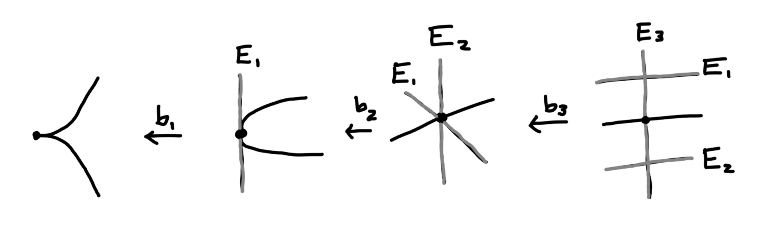
\includegraphics[scale=0.6]{log_resolution}
    \end{center}
    The singularity gives multiplicity two for $E_1$ when pulling back the
    curve, giving $E_1$ and $E_2$ discrepancy 0 and $E_3$ discrepancy $-1$.
    However for $\frac{5}{6}\{y^2=x^3\}$ the discrepancies are $\frac{2}{3}$ and
    $\frac{1}{2}$ for $E_1$ and $E_2$, so $E_3$ gets discrepancy 0 and
    $(\A^2,\frac{5}{6}\{y^2=x^3\})$ is log canonical. Hence
    $\frac{5}{6}\le\lct(\A^2;\{y^2=x^3\})\le1$.
\end{example}

\begin{theorem}[ACC for LCT; Hacon--McKernan--Xu]
    The set
    \begin{equation*}
        \LCT(n) = \{\lct(X;D)
            :\text{$\dim(X)=n$, $D$ an integral Weil divisor}\}
    \end{equation*}
    satisfies the ascending chain condition, i.e. if
    $\lambda_1\le\lambda_2\le\cdots$ is a sequence of values in $\LCT(n)$ then
    $\lambda_i=\lambda_{i-1}$ for $i\gg0$.
\end{theorem}

\section*{Adjunction}

\begin{proposition}[The adjunction formula]
    Let $D\subseteq X$ be a smooth divisor in a smooth variety. Then
    $\omega_X(D)|_D\cong\omega_D$, i.e. $(K_X+D)|_D\sim K_D$.
\end{proposition}

\begin{proof}[Proof 1]
    The short exact sequence $0\to T_D\to T_X|_D\to N_{D/X}\to0$ gives
    $\det T_D\otimes\det N_{D/X}\cong\det T_X|_D$, so
    $\omega_D^\vee\otimes N_{D/X}\cong \omega_X^\vee|_D$. Then note that
    $N_{D/X}\cong\O(D)|_D$.
\end{proof}

\begin{proof}[Proof 2]
    Near a point in $D$ choose coordinates $x_1,\ldots,x_n$ with $D=\{x_1=0\}$.
    Locally, a section of $\omega_X(D)$ is of the form
    $f\frac{dx_1}{x_1}\wedge dx_2\wedge\cdots\wedge dx_n$ where $f\in\O_X$. We
    define the Poincar\'e residue $\Res:\omega_X(D)|_D\to\omega_D$ by
    \begin{equation*}
        f\frac{dx_1}{x_1}\wedge dx_2\wedge\cdots\wedge dx_n
            \mapsto f|_D\cdot dx_2\wedge\cdots\wedge dx_n.
    \end{equation*}
    Note that this is in fact a well-defined map of sheaves. Locally, it is
    surjective since $\alpha\in\omega_D$ lifts to a form $dx_1/x_1\wedge\alpha$
    in $\omega_X(D)|_D$ with residue $\alpha$, and injective by construction, so
    it is an isomorphism of sheaves.
\end{proof}

If either of $X$ or $D$ is singular then this can fail.

\begin{example}
    Let $\F_n=\P(\O_{\P^1}\oplus\O_{\P^1}(n))$, the Hirzebruch surface. We have
    two rational curves $\Sigma_n=\P(\O_{\P^1})$ and
    $\Sigma_{-n}=\P(\O_{\P^1}(n))$ together with the fibers $F$ satisfying
    \begin{equation*}
        F^2=0, \qquad \Sigma_n^2=n, \qquad \Sigma_{-n}^2=-n, \qquad
        \Sigma_n\cdot\Sigma_{-n}=0, \qquad F\cdot\Sigma_{\pm n}=1.
    \end{equation*}
    For $n>0$, it is a fact that there exists a contraction $p:\F_n\to X$ of
    $\Sigma_{-n}$. Here $X$ turns out to be the cone over the degree $n$
    Veronese embedding of $\P^1$. Consider $C=p(F)$. To compute the log
    discrepancy, suppose
    \begin{equation*}
        p^*(K_X+C) + (a-1)\Sigma_{-n} = K_{\F_n} + F.
    \end{equation*}
    By the projection formula we have $\Sigma_{-n}\cdot p^*(K_X+C)=0$, since $p$
    contracts $\Sigma_{-n}$. On the other hand $\Sigma_{-n}\cdot K_{\F_n}=n-2$,
    since $(K_{\F_n}+\Sigma_{-n})\cdot\Sigma_{-n}=K_{\Sigma_{-n}}=-2$ by
    adjunction. Hence $n(1-a) =n-1$, so $a=1/n$. Now
    $(K_X+C)\cdot C=p^*(K_X+C)\cdot F$ by the projection formula, and so
    \begin{equation*}
        (K_X+C)\cdot C
            = (K_{\F_n}+F+(1-1/n)\Sigma_{-n})\cdot F
            = -2 + 0 + (1-1/n)
            \ne -2 = K_C.
    \end{equation*}
    Hence the adjunction formula fails for $C$ in $X$. In particular $X$ must be
    singular.
\end{example}

\begin{theorem}
    If $X$ is a normal variety, and $D\subset X$ is a normal reduced divisor,
    then
    \begin{equation*}
        (K_X+D)|_D = K_D + \Diff
    \end{equation*}
    where $\Diff$ is a canonically determined divisor on $D$, called the
    \emph{different}, such that
    \begin{enumerate}
        \item The different is effective; $\Diff\ge0$.

        \item ``Adjunction for singularities'': If $(X,D)$ is log canonical in a
            neighbourhood of $D$, then $(D,\Diff)$ is log canonical.

        \item ``Inversion of adjunction'': If $(D,\Diff)$ is log canonical, then
            $(X,D)$ is log canonical in a neighbourhood of $D$.
    \end{enumerate}
\end{theorem}

\begin{proof}[Sketch proof]
    Take a log resolution $p:(X',D')\to(X,D)$. Then
    \begin{equation*}
        p^*(K_X+D) = K_{X'}+D'+\Gamma
    \end{equation*}
    where $\Gamma$ is a $p$-exceptional divisor, and
    \begin{equation*}
        p^*(K_X+D)|_{D'} = (K_{X'}+D'+\Gamma)|_{D'} = K_{D'} + \Gamma|_{D'}
    \end{equation*}
    so we use $\Diff=p_*(\Gamma|_{D'})$.
    \begin{enumerate}
        \item Proof omitted; uses MMP.

        \item If $(X,D)$ is log canonical, let $p:(X',D')\to(X,D)$ be a log
            resolution. Then
            \begin{equation*}
                K_{X'} + D' + \sum E_i = p^*(K_X+D) + \sum a_iE_i
            \end{equation*}
            gives
            \begin{equation*}
                K_{D'} + \sum E_i|_{D'} = p^*(K_D+\Diff) + \sum a_iE_i|_{D'},
            \end{equation*}
            and $\sum E_i|_{D'}\ge\Diff'$, where $\Diff'$ is the strict
            transform of the different, because the different must have been
            blown up. Then
            \begin{equation*}
                K_{D'} + \Diff'
                    + \sum_{E_i\cap\Diff'=\emptyset}E_i|_{D'}
                    = p^*(K_D+\Diff) + \sum a_iE_i|_{D'},
            \end{equation*}
            so $(D,\Diff)$ is log canonical.

        \item This is a corollary of the following theorem:
    \end{enumerate}
\end{proof}

\begin{theorem}[Existence of log canonical modifications]
    Let $(X,\Delta)$ be a log pair. There exists a birational map
    $p:(X',\Delta')\to(X,\Delta)$, where $\Delta'$ is the strict transform of
    $\Delta$, such that
    \begin{enumerate}
        \item $(X',\Delta'+\exc(p))$ is log canonical.
        \item $K_{X'}+\Delta'+\exc(p)$ is $p$-ample.
        \item $K_{X'}+\Delta'+\exc(p)=p^*(K_X+\Delta)+F$ where $-F\ge0$, and if
            $F\ne0$ then every component of $\Delta'$ appears with a negative
            coefficient.
    \end{enumerate}
\end{theorem}

\begin{remark}
    The notion ``$p$-ample'' in 2 means that there is a divisor $G$ on $X$ such
    that $K_{X'}+\Delta'+\exc(p)+p^*G$ is ample. Note that 3 is a direct
    consequence of 2, and implies that the log discrepancies are zero if
    $(X,\Delta)$ is log canonical.
\end{remark}

\begin{proof}
    The proof is via the MMP, see [BCHM].
\end{proof}

\begin{proof}[Proof of inversion of adjunction]
    Consider the case $\Diff=0$. If $(X,D)$ is not log canonical, take a
    log canonical modification $\pi:(X',D')\to(X,D)$, so
    \begin{equation*}
        K_{X'} + D' + \exc(\pi) = \pi^*(K_X+D) + F
    \end{equation*}
    with $-F\ge0$. Since $(X,D)$ is not log canonical we must have $F\ne0$, so
    \begin{equation*}
        K_{D'} + \exc(\pi)|_{D'} = \pi^*(K_{D'}) + F|_{D'}
    \end{equation*}
    where $F|_{D'}\ne0$ because every component of $D'$ appears in $F$ with a
    negative coefficient. Hence $D'$ is not log canonical.
\end{proof}

\begin{corollary}
    Suppose $(X,\Delta)\to T$ is a fibration, where $\dim T=1$. If
    $(X_t,\Delta_t)$ is log canonical, then $(X,\Delta)$ is log canonical in a
    neighbourhood of $t$.
\end{corollary}

\begin{remark}
    Here a fibration means that $X\to T$ is a fibration (i.e. flat with
    connected fibres), and for all components $D$ of $\Supp\Delta$ the
    restriction $D\to T$ is also a fibration.
\end{remark}

\begin{remark}
    Hence log canonicity is an open condition on the base.
\end{remark}

It is a fact that KLT surface singularities are precisely the quotient
singularities. This is false in higher dimensions. There is even a
classification of log canonical singularities on surfaces, but in higher
dimensions the topology can be arbitrarily complicated.

\begin{exercise}
    If $X$ is a Calabi-Yau projective variety, show that the cone on $X$ is log
    canonical.
\end{exercise}

\section*{Moduli of curves}

The basic setup in moduli theory is a moduli functor:
\begin{equation*}
    F : \cat{Sch}_{k=\closure k}\to\cat{Set},
\end{equation*}
where
\begin{equation*}
    F(k) = \{\text{objects we want to parametrize}\},
\end{equation*}
e.g. curves. We need to decide what $F(T)$ is for general $T$.

The dream outcome is then
\begin{enumerate}[label=(\Roman*)]
    \item $F\cong_\Phi\Hom(-,\M)$ for some $\M$, so $k$-points of $\M$ are the
        objects we want to classify.
    \item There is a universal family $\U\to\M$ (the distinguished element of
        $F(\M)$) s.t. $s\in F(T)$, $\Phi(s):T\to M$ corresponds to a pullback
        family $\U\times_\M T\to T$.
\end{enumerate}
For example, for curves $\U\to\M$ should have fiber over a point of $\M$ given
by the corresponding curve. To ensure such an $\M$ exists we need to know what a
``good'' curve is (we can't hope to classify all curves), and also what a
``good'' \emph{family} of curves is, to define $F(T)$. Since a family of curves
is a morphism of relative dimension one, we think of the moduli of curves as
being really the moduli of morphisms of relative dimension one.

What ``goodness'' do we need?
\begin{enumerate}[label=\arabic*)]
    \item A positivity constraint (e.g. something being ample).
        For curves: $g\ge2$; $\omega_C$ ample.

    \item A singularity constraint. (We want $\M$ to be separated and proper.)
\end{enumerate}
So we care about singularities of morphisms.

\begin{definition}
    A morphism $f:X\to T$ where $T$ is a curve is \emph{locally stable} if it is
    flat, and $(X,f^{-1}(t))$ is (semi) log-canonical for all $t\in T$.
\end{definition}

By adjunction, this is equivalent to the fibres being (semi) log-canonical. (If
$\dim(X/T)=1$ this is equivalent to the fibres being nodal curves.)

\begin{definition}
    A morphism $f:X\to T$ is \emph{stable} if it is locally stable and $K_X$ is
    $f$-ample (i.e. $K_X+f^*D$ is ample for some $D$).
\end{definition}

Semi-stable implies stable, but the converse may fail: $f:\A^3\to\A^1$,
$(x,y,z)\mapsto x^3+y^3+z^3$ is locally stable but not semi-stable.

\begin{example}
    Fix $C$ of genus at least 2. Consider $C\times\A^1\to\A^1$, and blowup a
    single point on $C\times\{0\}$. Write $E$ for the exceptional divisor, which
    is a copy of $\P^1$, and $C'$ for the strict transform of $C$. We have
    $(C')^2=-1$, since $0=C^2$ so $(C'+E)^2=0$, and by Grauert / Artin we can
    contract $C'$ to a point. The result has a very bad singularity from $C'$,
    and is no longer locally stable.
\end{example}

If we allowed this family in our moduli functor, then the point corresponding to
$\P^1$ would be in the closure of the point corresponding to $C$. This would be
true for all such $C$, so $\M$ would be badly non-separated. Hence we need the
local stability condition for $\M$ to be separated.

Without the positivity condition, we can do a similar thing repeatedly blowing
up points on $C\times\A^1$ to get infinitely many distinct curves in the closure
of the point corresponding to $C$, which would prevent $\M$ from being finite
type.

\begin{theorem}
    Stable curves with fixed geometric genus form a good moduli space
    $\closure{\M_g}$.
\end{theorem}

(Due to recent work this is true for higher dimensional varieties if you replace
genus with volume.)

\begin{theorem}
    The moduli space of stable curves is separated and proper.
\end{theorem}

\begin{proof}
    For properness, use the valuative criterion:
    \begin{equation*}
        \begin{tikzcd}[column sep=huge]
            X^0 \ar[d,"\text{stable family}"'] \ar[r,dashed] & X \ar[d] \\
            C^0 \ar[r,hook] & C.
        \end{tikzcd}
    \end{equation*}
    We want to complete a stable family over $C^0=C\setminus\{p\}$ to a stable
    family over $C$.
    \begin{itemize}
        \item Step 1: Complete $X^0$ to some family $Y\to C$ (e.g. embed in
            projective space over $C$ and take closure).

        \item Step 2: Take a semi-stable reduction of $Y\to C$.
            \begin{equation*}
                \begin{tikzcd}[column sep=huge]
                    Y' \ar[r,"\text{bir.}"] \ar[dr,"g","\text{semi-stable}"'] &
                    Y\times_CC' \ar[d] & Y \ar[d] \\
                                       & C' \ar[r,"\text{finite}"] & C.
                \end{tikzcd}
            \end{equation*}
            (Finite base-change is allowed, stack not a scheme.) Then $Y'\to C'$
            is locally stable, but $K_{Y'}$ may not be ample over $C'$.

        \item Step 3: We want to restore ampleness by contracting all curves $E$
            in $Y'$ s.t. $g(E)$ is a point and $K_{Y'}\cdot E\le0$. This can be
            fixed by the MMP.
    \end{itemize}
    For separatedness (uniqueness of lifts) we use uniqueness from MMP.
\end{proof}

If $C$ is a stable curve, then $\omega_C^{\otimes 3}$ is very ample, and as an
exercise one can check that $h^0(\omega_C^{\otimes 3})=5g-5$. Choosing a basis
$\{\sigma_i\}$ for $H^0(\omega_C^{\otimes 3})$ gives an embedding
$C\hookrightarrow\P^{5g-6}$, so every stable curve embeds with degree $6g-6$ in
$\P^{5g-6}$. Hence there is a component of the Hilbert scheme $H$ of $\P^{5g-6}$
containing all these curves.

\paragraph{Problem 1.} $H$ has points not corresponding to stable curves.

\paragraph{Problem 2.} This presentation depends on the choice of basis, so each
stable curves appears many times in $H$. (The stabilizer is $\PGL(5g-5)$.)

~

So we want a suitable open locus within a suitable quotient $H/\PGL(5g-5)$.
Mumford developed ``geometric invariant theory'' (GIT), which defines a subset
$H^s\subseteq H$ of ``GIT stable'' points, and a Deligne-Mumford stack
$H^s\sslash\PGL(5g-5)$ which is a suitable quotient of $H$ by $\PGL(5g-5)$. As a
miracle, the set of GIT stable points $H^s$ is precisely the set of points
corresponding to stable curves. In higher dimensions this doesn't hold.

\end{document}
